\documentclass[../../main.tex]{subfiles}
\begin{document}

{\bf [解]}

\paragraph{(1)}
$A$ に赤玉が $x$ 個入っている時，1回試行をして，$A$ の赤玉が1つ増える確率 $\alpha_x$，変化しない確率 $\beta_x$，1つ減る確率 $\gamma_x$ とおく．

% ========================================================
% 1. 試行における玉の取り出しと戻しの分岐フロー図 (手描き図の清書)
% ========================================================
\begin{figure}[htb]
  \centering
  \begin{tikzpicture}[
      >=stealth,
      node distance=1.2cm and 2.5cm,
      every node/.style={font=\small},
      branch/.style={circle, fill=gray!80, inner sep=1.2pt},
      box/.style={rectangle, rounded corners=3pt, draw=gray!70, thick, fill=white, inner sep=4pt}
    ]

    % --- 左端ノード (A からの取り出し) ---
    \node[box, draw=red!70!black] (RedPick) at (0, 1.3) {$A$ から赤を取る $\left(\dfrac{x}{4}\right)$};
    \node[box, draw=gray!70!black] (WhitePick) at (0, -1.3) {$A$ から白を取る $\left(\dfrac{4-x}{4}\right)$};

    % --- 右端ノード (A への戻し) ---
    \node[right=2.2cm of RedPick, yshift=0.8cm] (RtoR) {$A$ に赤を戻す};
    \node[right=2.2cm of RedPick, yshift=-0.8cm] (RtoW) {$A$ に白を戻す};

    \node[right=2.2cm of WhitePick, yshift=0.8cm] (WtoR) {$A$ に赤を戻す};
    \node[right=2.2cm of WhitePick, yshift=-0.8cm] (WtoW) {$A$ に白を戻す};

    % --- 矢印の接続 ---
    \draw[->, thick, red!80!black] (RedPick.east) -- (RtoR.west);
    \draw[->, thick, red!80!black] (RedPick.east) -- (RtoW.west);

    \draw[->, thick, gray!80!black] (WhitePick.east) -- (WtoR.west);
    \draw[->, thick, gray!80!black] (WhitePick.east) -- (WtoW.west);

    % --- 確率の計算式と赤玉個数の変化 ---
    \node[right=0.2cm of RtoR] {$\dots \dfrac{x}{4} \left[ \dfrac{1}{2} + \dfrac{1}{2} \cdot \dfrac{2}{3} \right] = \dfrac{5}{6} \dfrac{x}{4}$ \quad \textbf{(変化なし)}};
    \node[right=0.2cm of RtoW] {$\dots \dfrac{x}{4} \left[ 0 + \dfrac{1}{2} \cdot \dfrac{1}{3} \right] = \dfrac{1}{6} \dfrac{x}{4}$ \quad \textcolor{blue!80!black}{\textbf{($-1$ 減少)}}};

    \node[right=0.2cm of WtoR] {$\dots \dfrac{4-x}{4} \left[ \dfrac{1}{2} \cdot \dfrac{2}{3} + \dfrac{1}{2} \cdot \dfrac{1}{3} \right] = \dfrac{1}{2} \dfrac{4-x}{4}$ \quad \textcolor{red!80!black}{\textbf{($+1$ 増加)}}};
    \node[right=0.2cm of WtoW] {$\dots \dfrac{4-x}{4} \left[ \dfrac{1}{2} \cdot \dfrac{1}{3} + \dfrac{1}{2} \cdot \dfrac{2}{3} \right] = \dfrac{1}{2} \dfrac{4-x}{4}$ \quad \textbf{(変化なし)}};

  \end{tikzpicture}
  \caption{1回の試行における玉の取り出しと戻しの分岐フロー}
  \label{fig:ball_branch_flow}
\end{figure}

% ========================================================
% 2. 赤玉の個数の状態遷移図 (alpha_x, beta_x, gamma_x)
% ========================================================
\begin{figure}[htb]
  \centering
  \begin{tikzpicture}[>=stealth, scale=1.3, every node/.style={font=\small}]

    % --- 状態ノード ---
    \node[circle, thick, fill=blue!10, minimum size=1.1cm] (Xminus) at (0, 0) {$x-1$};
    \node[circle, very thick, fill=yellow!20, minimum size=1.2cm] (X) at (4, 0) {$x$};
    \node[circle, thick, fill=red!10, minimum size=1.1cm] (Xplus)  at (8, 0) {$x+1$};

    % --- 1. 増加遷移 (x -> x+1: alpha_x) ---
    \draw[->, very thick, red!80!black] (X) to[bend left=30]
    node[above, font=\footnotesize] {$\alpha_x = \dfrac{4-x}{8}$} (Xplus);

    % --- 2. 減少遷移 (x -> x-1: gamma_x) ---
    \draw[->, very thick, blue!80!black] (X) to[bend left=30]
    node[above, font=\footnotesize] {$\gamma_x = \dfrac{x}{24}$} (Xminus);

    % --- 3. 自状態維持ループ (x -> x: beta_x) ---
    \draw[->, very thick, green!60!black] (X) to[out=120, in=60, looseness=5]
    node[above=2pt, font=\footnotesize] {$\beta_x = \dfrac{6+x}{12}$} (X);

    % --- 逆向きの流入矢印（漸化式の構成イメージ） ---
    \draw[->, dashed, gray!70] (Xminus) to[bend right=30]
    node[below, font=\scriptsize] {$\alpha_{x-1} = \dfrac{5-x}{8}$} (X);
    \draw[->, dashed, gray!70] (Xplus) to[bend right=30]
    node[below, font=\scriptsize] {$\gamma_{x+1} = \dfrac{x+1}{24}$} (X);

  \end{tikzpicture}
  \caption{赤玉の個数 $x$ に関する状態遷移図}
  \label{fig:state_transition_diagram}
\end{figure}

上の遷移図から，
\begin{align}
  \alpha_x &= \dfrac{1}{2} \dfrac{4-x}{4}, \\
  \beta_x &= \dfrac{5}{6} \dfrac{x}{4} + \dfrac{1}{2} \dfrac{4-x}{4} = \dfrac{6+x}{12}, \\
  \gamma_x &= \dfrac{x}{24}
\end{align}
であるから，$n+1$ 回目の試行の後に $A$ に赤い玉が入っている確率$P_{n+1}(x)$は，$n$ 回目の個数 $x, x \pm 1$ で場合分けして
\begin{align}
  P_{n+1}(x)
  &= \dfrac{6+x}{12} P_n(x) + \dfrac{x+1}{24} P_n(x+1) + \dfrac{4-(x-1)}{8} P_n(x-1) \\
  &= \dfrac{1}{12}(6+x) P_n(x) + \dfrac{1}{24}(x+1) P_n(x+1) + \dfrac{1}{8}(5-x) P_n(x-1) \label{eq:1}
\end{align}
となる．よって題意は示された．

\paragraph{(2)}

\cref{eq:2}の両辺に$x$を書けると
\begin{align}
  x P_{n+1}(x) = \dfrac{1}{12} x (6+x) P_n(x) + \dfrac{x}{24} (x+1) P_n(x+1) + \dfrac{1}{8} x (5-x) P_n(x-1)
\end{align}
であるから，$x = 0, 1, 2, 3, 4, 5$ として足し合わせると
\begin{align}
  E_{n+1} &= \dfrac{1}{12} \sum_{x=0}^5 (6x P_n(x) + x^2 P_n(x)) \\
  &\qquad + \dfrac{1}{24} \sum_{x=0}^5 \{(x+1)^2 P_n(x+1) - (x+1) P_n(x+1)\} \\
  &\qquad + \dfrac{1}{8} \sum_{x=0}^5 \{-(x-1)^2 P_n(x-1) + 3(x-1) P_n(x-1) + 4 P_n(x-1)\} \label{eq:2}
\end{align}
となる．

以下各項計算する． 簡単のため$T = \sum_{x=1}^4 x^2 P_n(x)$ とする．$P_n(5) = 0$に注意して
\begin{align}
  \dfrac{1}{12} \sum_{x=0}^5 (6x P_n(x) + x^2 P_n(x)) = \dfrac{1}{12} [ 6 E_n + T ] \\
  \dfrac{1}{24} \sum_{x=0}^5 \{(x+1)^2 P_n(x+1) - (x+1) P_n(x+1)\} = \dfrac{1}{24} [ T - E_n ] \\
  \dfrac{1}{8} \sum_{x=0}^5 \{-(x-1)^2 P_n(x-1) + 3(x-1) P_n(x-1) + 4 P_n(x-1)\} = \dfrac{1}{8} [ -T + 3 E_n + 4 ] \quad (\because \sum_{x=0}^4 P_n(x) = 1)
\end{align}
を得る．これらを\cref{eq:2}に代入して$E_{n}$についての漸化式は
\begin{align}
  E_{n+1} &= \dfrac{20}{24} E_n + \dfrac{1}{2} = \dfrac{5}{6} E_n + \dfrac{1}{2}
  \therefore
  E_{n+1} - 3 &= \dfrac{5}{6} (E_n - 3) \label{eq:3}
\end{align}
となる．

初項について考える．はじめ$A$ には赤1個と白3個が入っていたので$E_0 = 1$であるから，\cref{eq:3}より
\begin{align}
  E_n = \Bigl(\dfrac{5}{6}\Bigr)^n (1 - 3) + 3 = 3 - 2 \Bigl(\dfrac{5}{6}\Bigr)^n \label{eq:4}
\end{align}
である．

\paragraph{(3)}
\cref{eq:4}で$n\to\infty$の極限をとって
\begin{align}
  \lim_{n\to\infty} E_n = 3
\end{align}
である．

\end{document}
